\documentclass[11pt]{article}
\usepackage[margin=1in]{geometry}
\usepackage{pgfplots}
\pgfplotsset{compat=1.18}
\usepgfplotslibrary{groupplots}
\usepackage{booktabs}
\usepackage{amsmath}
\usepackage{xcolor}
\usepackage{caption}
\usepackage[hidelinks]{hyperref}
\usepackage{enumitem}

\definecolor{cdense}{HTML}{1B6CA8}
\definecolor{cmoe}{HTML}{C0392B}
\definecolor{cfd}{HTML}{27AE60}
\definecolor{cmtp}{HTML}{8E44AD}

\title{\textbf{DFlash speculative decoding on 2\,$\times$\,Tesla V100:\\
a controlled dense-vs-MoE sweep, and why the MoE regression is Amdahl, not acceptance}}
\author{Hsiu-Chi Tsai \\ \texttt{thc1006}}
\date{July 2026}

\begin{document}
\maketitle

\begin{abstract}
\noindent
On \textbf{2\,$\times$\,Tesla V100 32\,GB (sm\_70)} with \texttt{llama.cpp b9860} built for Volta, I ran a single-rig,
quantization-matched sweep of \href{https://z-lab.ai/projects/dflash/}{DFlash} block-diffusion speculative decoding
(\href{https://github.com/ggml-org/llama.cpp/pull/22105}{PR \#22105}, \href{https://github.com/ggml-org/llama.cpp/issues/25117}{issue \#25117})
over \verb|--spec-draft-n-max|, for a \emph{dense} target (Qwen3.6-27B) and an \emph{MoE} target (Qwen3.6-35B-A3B), plus a fast-dense
control and an MTP comparison. DFlash speedup peaks at a \emph{low} $n$ ($\approx 2\text{--}4$) and erodes as $n$ grows for
\emph{both} architectures; the MoE crosses into net-loss earlier. Crucially, \textbf{draft acceptance is near-identical between dense
and MoE at every $n$} while their baselines differ $2.57\times$, so the MoE weakness on a cleanly-quantized target is \emph{not} a
draft-acceptance deficit. A cost decomposition and a fast-dense control point to an \textbf{Amdahl effect on the drafter} (a faster
baseline makes the drafter/verify overhead a larger fraction of the per-token budget) rather than the expert-union mechanism assumed
in the thread---though expert-activation counts were not measured, so expert-union is neither tested nor excluded. MTP beats DFlash
across the swept range. \textbf{All magnitudes are V100-class only and throughput-only (quality was not evaluated).}
\end{abstract}

\section{Context and what is new}
The \#25117 thread reports that DFlash regresses on quantized MoE targets and asks how to raise MoE acceptance. Community datapoints
exist but are scattered across different hardware, quantizations, and single configurations: @andyskw swept dense-27B on an iGPU;
@gelim measured MTP vs.\ DFlash on V100 dense; @jschmied found the peak at $n{=}3\text{--}4$; @jerrydong1988 filed the original MoE
regression; @ruixiang63 (the PR author) documented gpt-oss MoE underperformance and hypothesized \emph{expert-union} (a larger verify
block activates more experts). What is missing---and what this note adds---is a \textbf{paired dense-and-MoE sweep on one rig at
matched quantization}, so that acceptance can be compared apples-to-apples and the mechanism separated from confounds.

\section{Setup}
\textbf{Hardware/build.} 2\,$\times$\,V100 32\,GB (sm\_70); \texttt{b9860} built from source for \texttt{sm\_70} via a user-space
conda CUDA~12.4 (official prebuilt CUDA drops Volta). \textbf{Targets (matched quant IQ4\_XS)}: Qwen3.6-27B (dense) and
Qwen3.6-35B-A3B (MoE); DFlash drafters both Q8\_0. \textbf{Controls}: a fast-dense Qwen3-4B (base 147.9~tok/s, drafter self-converted
from z-lab source), and MTP via the native \texttt{nextn} head of a Qwen3.6-27B MTP GGUF. \textbf{Protocol}: \texttt{llama-server},
\texttt{/v1/chat/completions}, \texttt{-fa on -ngl 99 -ngld 99}; \textbf{non-thinking} primary regime (real answer tokens, the
production-chat regime); \textbf{fixed budget} \texttt{ignore\_eos, n\_predict=384} (both sides emit 384 real tokens $\Rightarrow$ fair
paired timing); greedy headline plus a \texttt{temp 0.7} pass; \textbf{40 generative prompts} in 6 categories; \textbf{randomized}
config order; each config a fresh single-stream server. Paired per-prompt geometric-mean speedup with 10k-sample bootstrap 95\% CIs.
Full details, exact commands, and the reproducer are in the accompanying repository.

\section{Results}

\begin{figure}[h]
\centering
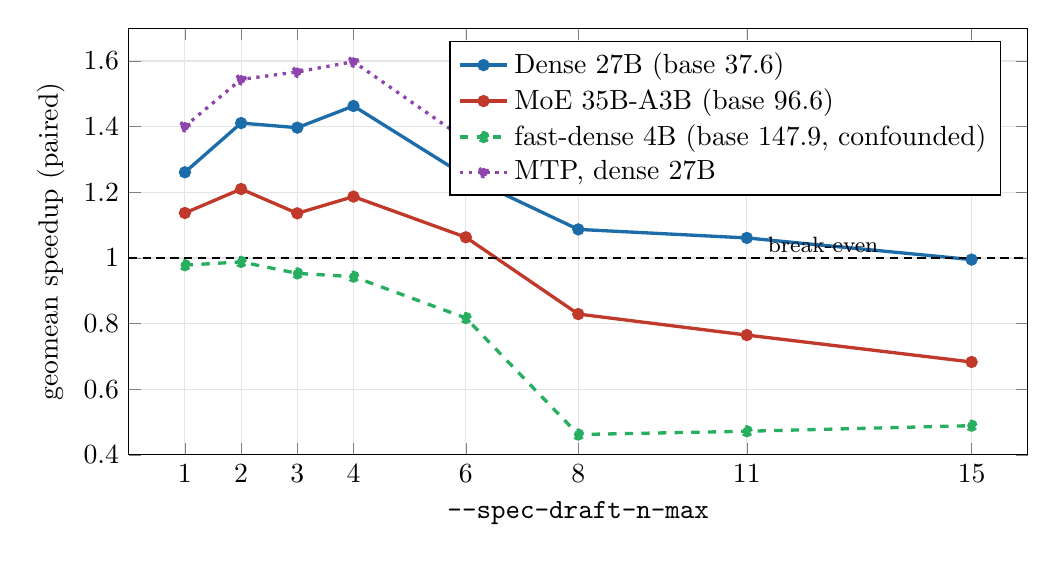
\begin{tikzpicture}
\begin{axis}[width=13cm,height=7cm,xlabel={\texttt{--spec-draft-n-max}},ylabel={geomean speedup (paired)},
  xmin=0,xmax=16,ymin=0.4,ymax=1.7,xtick={1,2,3,4,6,8,11,15},grid=both,grid style={gray!20},
  legend pos=north east,legend cell align=left,every axis plot/.append style={very thick,mark=*,mark size=1.6pt}]
\addplot[cdense] coordinates {(1,1.261)(2,1.411)(3,1.397)(4,1.463)(6,1.249)(8,1.087)(11,1.061)(15,0.995)};
\addlegendentry{Dense 27B (base 37.6)}
\addplot[cmoe] coordinates {(1,1.137)(2,1.210)(3,1.136)(4,1.187)(6,1.063)(8,0.829)(11,0.765)(15,0.683)};
\addlegendentry{MoE 35B-A3B (base 96.6)}
\addplot[cfd,dashed] coordinates {(1,0.978)(2,0.988)(3,0.953)(4,0.943)(6,0.817)(8,0.462)(11,0.472)(15,0.489)};
\addlegendentry{fast-dense 4B (base 147.9, confounded)}
\addplot[cmtp,dotted] coordinates {(1,1.401)(2,1.544)(3,1.567)(4,1.598)(6,1.360)};
\addlegendentry{MTP, dense 27B}
\draw[black,densely dashed] (axis cs:0,1) -- (axis cs:16,1);
\node[anchor=west,font=\footnotesize] at (axis cs:11.2,1.04) {break-even};
\end{axis}
\end{tikzpicture}
\caption{Speedup vs.\ draft depth. Both architectures peak at low $n$ and erode; the MoE (faster baseline) crosses break-even
earlier. The fast-dense 4B---no experts---erodes hardest, consistent with a baseline-speed effect (but it is confounded;
\S\ref{sec:mech}). MTP dominates DFlash across the swept range.}
\label{fig:speedup}
\end{figure}

\begin{table}[h]
\centering\small
\caption{DFlash speedup (geomean [95\% CI]) and pooled draft acceptance, non-thinking greedy, matched IQ4\_XS.}
\begin{tabular}{r rr rr}
\toprule
& \multicolumn{2}{c}{Dense 27B} & \multicolumn{2}{c}{MoE 35B-A3B}\\
\cmidrule(lr){2-3}\cmidrule(lr){4-5}
$n$ & geomean [CI] & accept & geomean [CI] & accept\\
\midrule
1  & 1.261 [1.24,1.28] & 84.1\% & 1.137 [1.12,1.15] & 82.4\%\\
2  & 1.411 [1.37,1.46] & 72.5\% & 1.210 [1.17,1.25] & 69.2\%\\
3  & 1.397 [1.33,1.46] & 61.0\% & 1.136 [1.08,1.19] & 58.8\%\\
4  & \textbf{1.463} [1.37,1.56] & 52.8\% & \textbf{1.187} [1.11,1.27] & 50.9\%\\
6  & 1.249 [1.15,1.35] & 39.8\% & 1.063 [0.97,1.16] & 38.5\%\\
8  & 1.087 [0.99,1.19] & 31.2\% & \textbf{0.829} [0.75,0.91] & 30.3\%\\
11 & 1.061 [0.96,1.18] & 23.5\% & 0.765 [0.69,0.85] & 22.6\%\\
15 & 0.995 [0.89,1.11] & 17.4\% & 0.683 [0.61,0.77] & 16.6\%\\
\bottomrule
\end{tabular}
\label{tab:main}
\end{table}

\paragraph{It is not an acceptance problem.} Figure~\ref{fig:accept} overlays the acceptance curves: dense and MoE are
near-identical at every $n$ (dense marginally higher, $+0.7$ to $+3.3$\,pp) even though the baselines differ $2.57\times$. For a
cleanly-quantized MoE, then, ``raise the draft acceptance rate'' is not the missing lever---the MoE drafts about as well as the dense
model; the loss is on the throughput/overhead side. (The OP's target is a much heavier-quantized 122B-A10B where a quant/feature
mismatch could \emph{additionally} depress acceptance---a separate axis this matched-quant pair does not isolate.)

\begin{figure}[h]
\centering
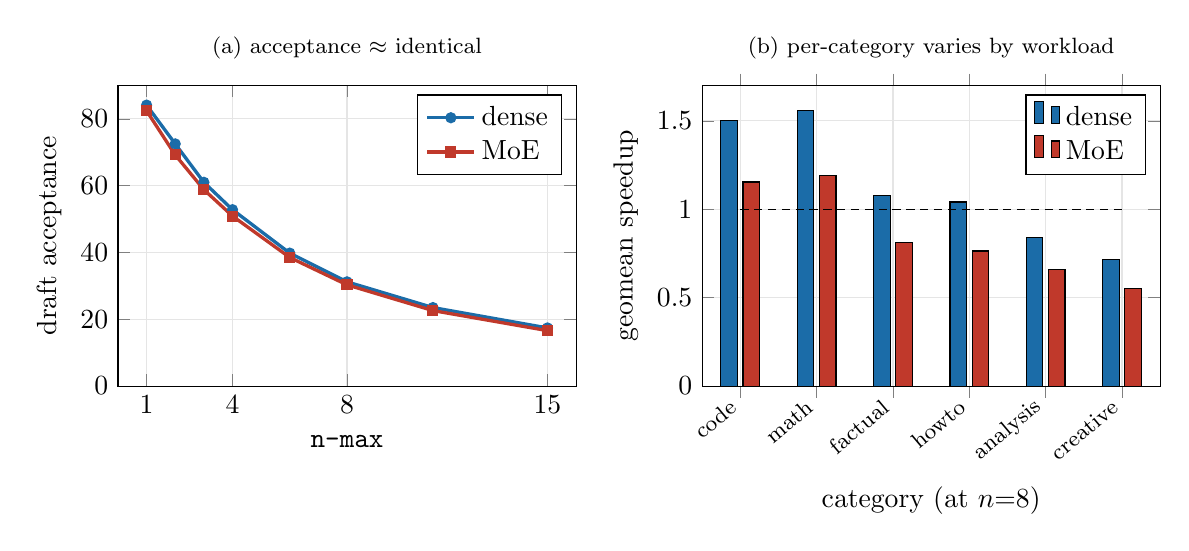
\begin{tikzpicture}
\begin{groupplot}[group style={group size=2 by 1,horizontal sep=1.6cm},width=7.4cm,height=5.4cm]
\nextgroupplot[xlabel={\texttt{n-max}},ylabel={draft acceptance},xmin=0,xmax=16,ymin=0,ymax=90,
  xtick={1,4,8,15},grid=both,grid style={gray!20},legend pos=north east,legend cell align=left,
  title={\footnotesize (a) acceptance $\approx$ identical}]
\addplot[cdense,very thick,mark=*,mark size=1.4pt] coordinates {(1,84.1)(2,72.5)(3,61.0)(4,52.8)(6,39.8)(8,31.2)(11,23.5)(15,17.4)};
\addlegendentry{dense}
\addplot[cmoe,very thick,mark=square*,mark size=1.4pt] coordinates {(1,82.4)(2,69.2)(3,58.8)(4,50.9)(6,38.5)(8,30.3)(11,22.6)(15,16.6)};
\addlegendentry{MoE}
\nextgroupplot[ybar,bar width=6pt,xlabel={category (at $n{=}8$)},ylabel={geomean speedup},
  symbolic x coords={code,math,factual,howto,analysis,creative},xtick=data,x tick label style={rotate=40,anchor=east,font=\footnotesize},
  ymin=0,ymax=1.7,grid=both,grid style={gray!20},legend pos=north east,legend cell align=left,
  title={\footnotesize (b) per-category varies by workload}]
\addplot[fill=cdense] coordinates {(code,1.501)(math,1.560)(factual,1.080)(howto,1.041)(analysis,0.839)(creative,0.717)};
\addlegendentry{dense}
\addplot[fill=cmoe] coordinates {(code,1.154)(math,1.193)(factual,0.812)(howto,0.764)(analysis,0.661)(creative,0.550)};
\addlegendentry{MoE}
\draw[black,densely dashed] (axis cs:code,1) -- (axis cs:creative,1);
\end{groupplot}
\end{tikzpicture}
\caption{(a) Draft acceptance is near-identical between dense and MoE at every $n$, so draftability is not the differentiator.
(b) Per-category speedup at $n{=}8$ varies widely by workload in both models (code/math draft well; creative/analysis do not), so a single
``average speedup'' depends on the prompt mix.}
\label{fig:accept}
\end{figure}

\section{Mechanism: Amdahl on the drafter}\label{sec:mech}
With acceptance held roughly equal, the dense-vs-MoE gap must be a per-step \emph{cost} effect. Define
$C(n)=\tau/\text{speedup}=T_{\text{step}}/T_{\text{base}}$, the per-step cost in units of a baseline decode token, where $\tau$ is the
mean accepted length per verify step. A linear fit $C(n)=d+v\,n$ gives a \textbf{near-equal fixed intercept} ($d\approx1.5$ for both;
batched verification costs $\approx1.5\times$ a single decode) but a \textbf{marginal cost $v$ that rises with baseline speed}
(Fig.~\ref{fig:amdahl}). In \emph{absolute} milliseconds the MoE's per-draft-token cost is actually \emph{lower}; it only looks worse
once normalized by its $2.57\times$ faster baseline. That is an Amdahl effect: the same overhead is a larger fraction of a cheaper
per-token budget, so the faster-baseline model crosses break-even at lower $n$. A fast dense model (Qwen3-4B, no experts) crosses
hardest of all, which is what a baseline-speed story predicts.

\textbf{What this does and does not show.} The fast-dense control is \emph{confounded}---it runs single-GPU (vs.\ 2-GPU tensor-split
for the big models), has $\sim$15\,pp lower acceptance, and uses a self-converted drafter---so it is suggestive only; the clean
evidence is the internal dense-vs-MoE contrast (equal acceptance, MoE's absolute cost not inflated). \textbf{I did not measure
expert-activation counts}, so this neither tests nor excludes the expert-union mechanism in the PR description; it only shows the
dense-vs-MoE ordering can be reproduced without it. Isolating any residual MoE-specific term would need a dense target matched to the
MoE's baseline speed, or direct expert-activation instrumentation.

\begin{figure}[h]
\centering
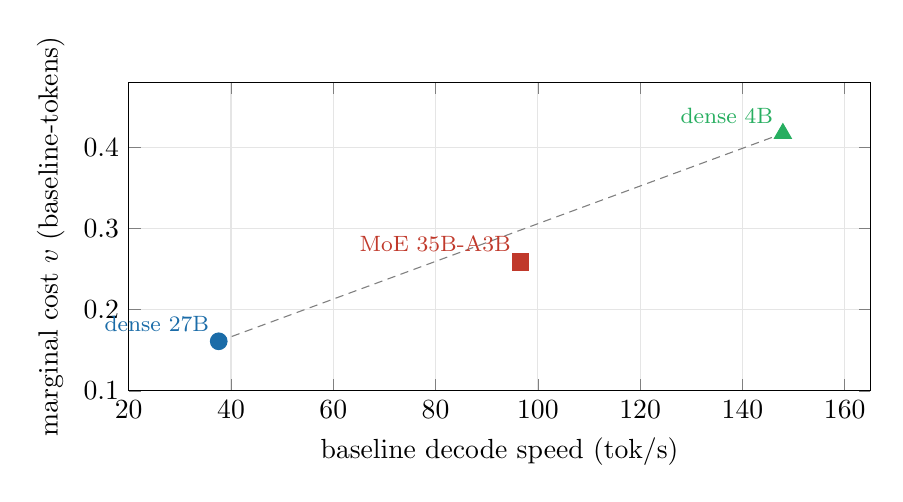
\begin{tikzpicture}
\begin{axis}[width=11cm,height=5.5cm,xlabel={baseline decode speed (tok/s)},ylabel={marginal cost $v$ (baseline-tokens)},
  xmin=20,xmax=165,ymin=0.1,ymax=0.48,grid=both,grid style={gray!20},
  nodes near coords,point meta=explicit symbolic,every node near coord/.append style={font=\footnotesize,anchor=south east}]
\addplot[only marks,mark=*,mark size=3pt,cdense] coordinates {(37.6,0.161)[dense 27B]};
\addplot[only marks,mark=square*,mark size=3pt,cmoe] coordinates {(96.6,0.259)[MoE 35B-A3B]};
\addplot[only marks,mark=triangle*,mark size=3.5pt,cfd] coordinates {(147.9,0.417)[dense 4B]};
\addplot[gray,densely dashed,domain=37.6:147.9,samples=2]{0.161+(0.417-0.161)/(147.9-37.6)*(x-37.6)};
\end{axis}
\end{tikzpicture}
\caption{Marginal per-step cost $v$ (in baseline-token units) rises monotonically with baseline decode speed across three models
(two dense, one MoE). Because the \emph{absolute} marginal cost is flat-to-lower for the faster models, the rise is the
$1/T_{\text{base}}$ (Amdahl) denominator, not a growing per-step cost. The expert-free 4B lying on the same trend argues the ordering
is baseline-speed, not MoE-architecture (control is confounded; treat as suggestive).}
\label{fig:amdahl}
\end{figure}

\section{Regime, sampling, and MTP}
\textbf{Thinking vs.\ non-thinking.} Thinking traces draft \emph{better} (higher acceptance and speedup at every tested $n$, both
models): e.g.\ dense $n{=}8$ rises $1.09\to1.23$, MoE $0.83\to0.90$. So the non-thinking (chat) numbers here are a \emph{lower bound}
for reasoning-heavy use. \textbf{Sampling.} \texttt{temp 0.7} $\approx$ greedy: a $1\text{--}3\%$ penalty, crossover unchanged.
\textbf{MTP} (native \texttt{nextn}) beats DFlash at every tested $n$ on the dense target (Fig.~\ref{fig:speedup}; $n{=}4$: MTP
$1.60\times$ vs.\ DFlash $1.46\times$), with higher acceptance too---consistent with an Amdahl reading, since the \texttt{nextn} head
is a near-free drafter that reuses the target forward. This matches @gelim (V100 dense, MTP $2.0\times>$ DFlash $1.65\times$) and
@jerrydong1988 (Strix-Halo MoE), now as a full sweep.

\section{Caveats}
\begin{itemize}[leftmargin=1.4em,itemsep=1pt]
\item \textbf{V100-class only.} Magnitudes and the crossover $n$ are bandwidth-dependent; do not extrapolate (the PR author reports
$2.69\times$ for the same dense model on a DGX Spark).
\item \textbf{Throughput only.} Greedy DFlash is not bit-identical to plain greedy under 2-GPU tensor-split (FP reduction order) $+$
MoE routing; a single-GPU $n{=}1$ run was $40/40$ identical, so this is a placement/routing artifact, not a lossy acceptance rule
($p_{\min}{=}0$). Output quality was not evaluated.
\item \textbf{Fast-dense control confounded} (placement, acceptance, self-converted drafter): suggestive, not proof.
\item \textbf{Expert-activation not measured}: the Amdahl reading is a hypothesis; expert-union is not tested or excluded.
\item \textbf{Peak is a plateau}: dense $n{=}2/3/4$ CIs overlap; the crossover is a \emph{region} (dense net-neutral $n{=}8\text{--}15$,
MoE robust net-loss from $n{=}8$), not a single point. Single greedy sweep; 40 prompts + CIs (not run-to-run reps).
\end{itemize}

\section*{Data, code, and credits}
Raw per-request JSON, the analysis that regenerates every number, the harnesses, and the full per-category/CI tables are in the
accompanying repository. This is a datapoint alongside prior thread contributors, not a correction of anyone: @ruixiang63 (PR,
tables, expert-union hypothesis, DGX-Spark numbers), @andyskw (first dense sweep), @gelim (V100 MTP-vs-DFlash), @jschmied (low-$n$
peak), @HH1162 (MoE $n{=}16$ no-speedup), @jerrydong1988 (original \#25117 report).

\end{document}
